
\subsection{Visualisierungs-Phase} 
Nach vollständiger Beendigung der Scan-Phase ging es in der Entwicklung weiter mit der Visualisierungs-Phase. Die zuvor gespeicherten Objekte und 
deren Informationen werden dabei abgerufen und können jederzeit erneut visualisiert und im Raum platziert werden. Die folgende Darlegung der 
Frontend-Entwicklung der Visualisierungs-Phase gibt einen Einblick auf die Oberfläche dieser Phase und wie diese aufgebaut ist. Dadurch sind die 
zugrundeliegenden Informationen veranschaulicht, welche für die nachstehende Backend-Implementierung von Relevanz ist.   
\subsubsection{FrontEnd}
Bei der Visualisierungs-Phase gibt es prinzipiell eine Benutzeroberfläche, die diesen Use Case ausmacht. Unter eigentlicher Anwendung dieser Phase und 
deren \acs{GUI} befinden sich darüber hinaus weitere Benutzeroberflächen, die bereits in der Scan-Phase schon erläutert wurden. Darunter zum Beispiel 
die in Abbildung (\ref{pic:image_tracking}) zu entnehmende Markererkennungs-\acs{UI}, die ebenso Bestandteil der Visualisierungs-Phase ist. 
\\ 
Die primäre \acs{GUI} ist ähnlich zu der Benutzeroberfläche der Scan-Phase aufgebaut. Ein Fragment, welches das Livebild der Kamera repräsentiert, das 
sich über den ganzen Bildschirm erstreckt. Dadurch können die bereits in der Scan-Phase erstellten Objekte erneut angezeigt werden. Des Weiteren befinden 
sich auf dieser Oberfläche zwei Buttons, zum einen zur Navigation, um auf das Startmenü zu gelangen und zum anderen, um die Objekte von der Datenbank 
abzugreifen, rendern und auf dem Bildschirm anzeigen zu lassen. Diese befinden sich jeweils in der linken und rechten unteren Ecke des Bildschrims, wie 
der Abbildung \ref{pic:visual} zu entnehmen ist. 
\\ 
Da diese \acs{UI} nur als Ansicht der zu visualisierenden Objekte gedacht ist, stehen dem Nutzer nur eingeschränkt Interaktionen mit der Oberfläche zur 
Verfügung. Diese belaufen sich lediglich auf die zuvor genannten Buttons und die dynamisch erzeugten Schaltflächen der Objekte, um zu den einzelnen 
Darbietungen der Objekte mehrere Informationen zu erlangen. 
\begin{figure}[hbt!]
    \centering
    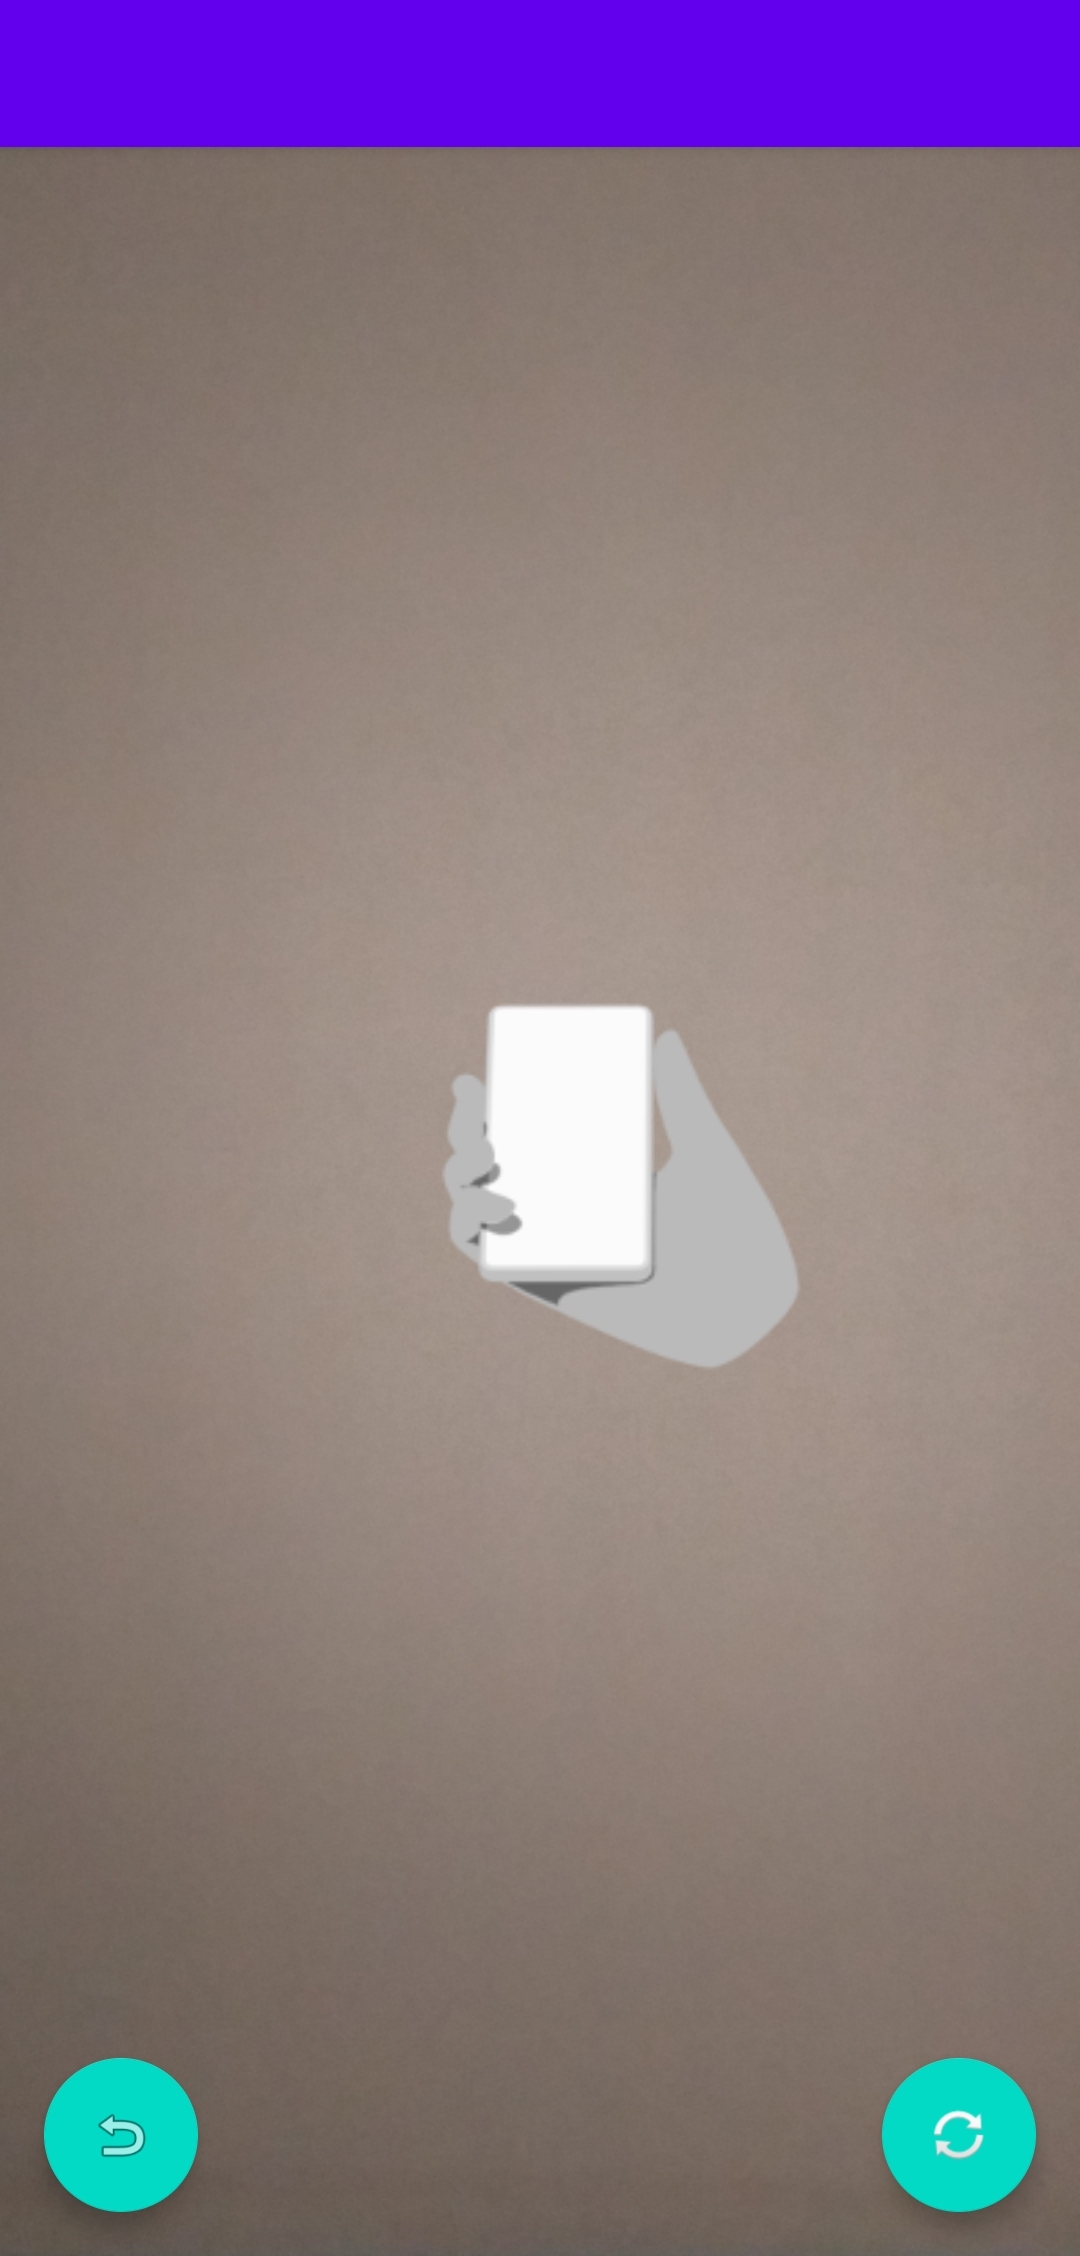
\includegraphics[width=10cm,height=7.5cm,keepaspectratio]{4Umsetzung/Bilder/visual-phase.jpg}
    \caption{Visualisierungs-Phase der Applikation}
    \label{pic:visual}
\end{figure}
\\ 
Nun erfolgt die Beschreibung der Backend-Implementierung und darüber hinaus werden Einblicke in die Programmierung der Visualisierungs-Phase gewährleistet. 
\subsubsection{BackEnd}

\section{Testdurchlauf / Test-Szenario}
\label{chap:testdurchlauf}